\documentclass{oblivoir}
\usepackage{amsmath,amssymb,amsthm,kotex,mdframed,paralist,kswrapfig}

\newcounter{num}
\newcommand{\prob}
{\bigskip\noindent\refstepcounter{num}\textbf{문제 \arabic{num})}\par}

\newcommand{\ans}{{\raggedleft\textbf{답 : (\qquad\qquad\qquad\qquad\qquad\qquad)}
\par}\bigskip\bigskip}


%%%
\begin{document}
\Large

\title{승재 18 - 6학년 2학기 - 11}
\author{}
\date{\today}
\maketitle
%\tableofcontents

\prob
다음과 같이 정육면체와 반원기둥으로 이루어진 입체도형의 겉넓이는 몇 cm\(^2\)입니까?
(원주율:3.1)

\begin{figure}[h!]
\centering
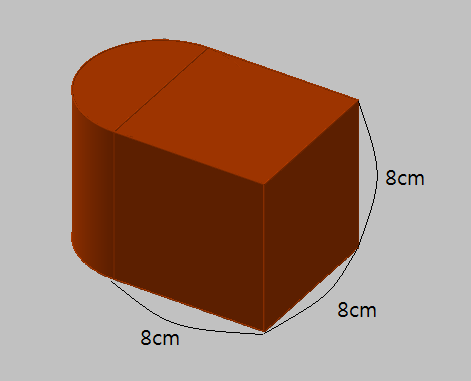
\includegraphics[width=0.6\textwidth]{01}
\end{figure}

\ans
\newpage

\prob
다음과 같이 정육면체와 반원기둥 두 개로 이루어진 입체도형의 겉넓이는 몇 cm\(^2\)입니까?
(원주율:3.1)

\begin{figure}[h!]
\centering
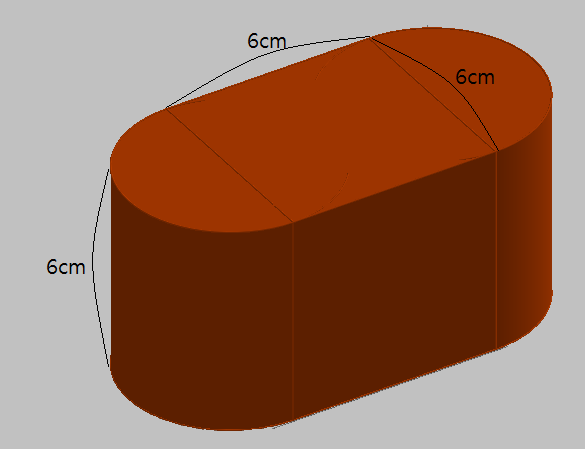
\includegraphics[width=0.6\textwidth]{02}
\end{figure}

\ans

\prob
다음과 같이 정육면체와 원기둥으로 이루어진 입체도형의 겉넓이는 몇 cm\(^2\)입니까?
(원주율:3.1)

\begin{figure}[h!]
\centering
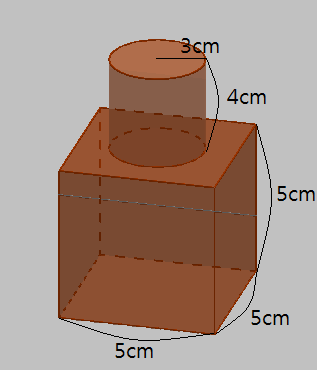
\includegraphics[width=0.4\textwidth]{03}
\end{figure}

\ans

\end{document}